\begin{figure}[H]
\centering
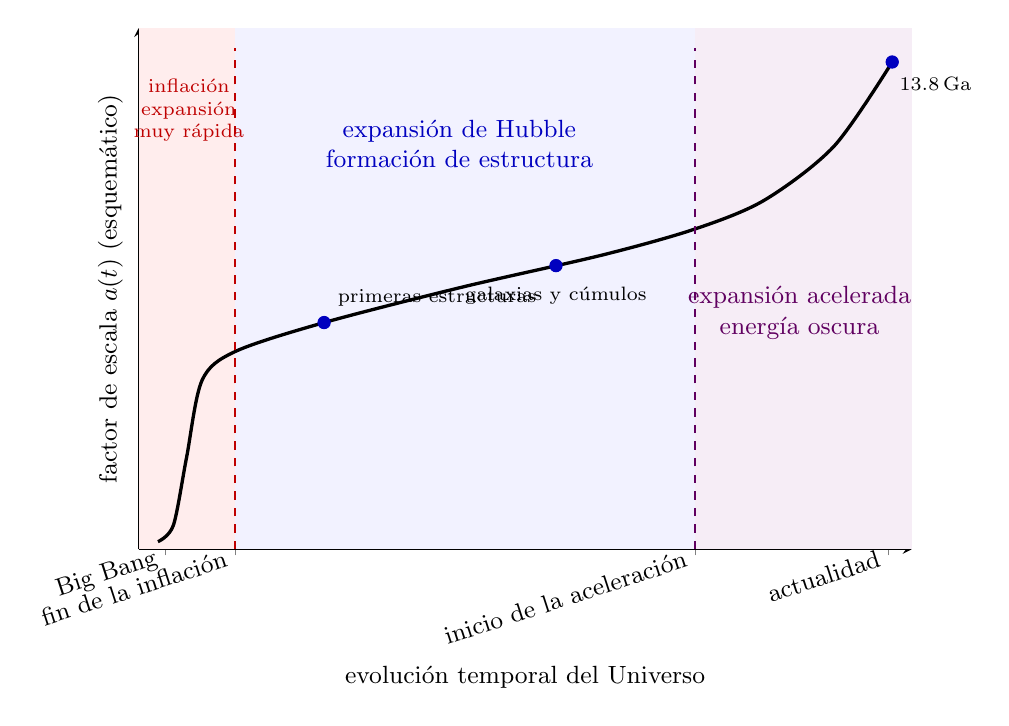
\begin{tikzpicture}
\begin{axis}[
    width=0.94\textwidth,
    height=8.2cm,
    xmin=0,
    xmax=10,
    ymin=0,
    ymax=5.4,
    axis lines=left,
    xlabel={evolución temporal del Universo},
    ylabel={factor de escala $a(t)$ (esquemático)},
    xtick={0.35,1.25,7.2,9.7},
    xticklabels={Big Bang,fin de la inflación,inicio de la aceleración,actualidad},
    ytick=\empty,
    tick label style={font=\small},
    label style={font=\small},
    x tick label style={rotate=18,anchor=east},
    clip=false
]
    \path[fill=red!7] (axis cs:0,0) rectangle (axis cs:1.25,5.4);
    \path[fill=blue!5] (axis cs:1.25,0) rectangle (axis cs:7.2,5.4);
    \path[fill=violet!7] (axis cs:7.2,0) rectangle (axis cs:10,5.4);

    \addplot[black,very thick,smooth]
        coordinates {
            (0.25,0.08)
            (0.45,0.25)
            (0.62,0.95)
            (0.82,1.75)
            (1.25,2.05)
            (2.4,2.35)
            (4.2,2.72)
            (6.0,3.05)
            (7.2,3.32)
            (8.1,3.62)
            (9.0,4.18)
            (9.75,5.05)
        };

    \addplot[red!75!black,thick,dashed]
        coordinates {(1.25,0) (1.25,5.2)};
    \addplot[violet!75!black,thick,dashed]
        coordinates {(7.2,0) (7.2,5.2)};

    \node[red!75!black,font=\scriptsize,align=center]
        at (axis cs:0.65,4.55) {inflación\\expansión\\muy rápida};
    \node[blue!75!black,font=\small,align=center]
        at (axis cs:4.15,4.2) {expansión de Hubble\\formación de estructura};
    \node[violet!75!black,font=\small,align=center]
        at (axis cs:8.55,2.45) {expansión acelerada\\energía oscura};

    \addplot[only marks,mark=*,mark size=2.2pt,blue!75!black]
        coordinates {(2.4,2.35) (5.4,2.94) (9.75,5.05)};
    \node[font=\scriptsize,anchor=south west]
        at (axis cs:2.45,2.42) {primeras estructuras};
    \node[font=\scriptsize,anchor=north]
        at (axis cs:5.4,2.82) {galaxias y cúmulos};
    \node[font=\scriptsize,anchor=west]
        at (axis cs:9.72,4.82) {$13.8\,\mathrm{Ga}$};
\end{axis}
\end{tikzpicture}
\caption{Representación esquemática de la historia de la expansión del Universo. La inflación corresponde a una expansión extremadamente rápida en el Universo temprano; después domina una etapa de expansión más gradual durante la cual se forman estructuras, y en tiempos recientes la expansión vuelve a acelerarse, fenómeno atribuido a la energía oscura. Las duraciones relativas de las etapas no están dibujadas a escala.}
\label{fig:expansion}
\end{figure}